\documentclass[man]{apa6}
\usepackage{lmodern}
\usepackage{amssymb,amsmath}
\usepackage{ifxetex,ifluatex}
\usepackage{fixltx2e} % provides \textsubscript
\ifnum 0\ifxetex 1\fi\ifluatex 1\fi=0 % if pdftex
  \usepackage[T1]{fontenc}
  \usepackage[utf8]{inputenc}
\else % if luatex or xelatex
  \ifxetex
    \usepackage{mathspec}
  \else
    \usepackage{fontspec}
  \fi
  \defaultfontfeatures{Ligatures=TeX,Scale=MatchLowercase}
\fi
% use upquote if available, for straight quotes in verbatim environments
\IfFileExists{upquote.sty}{\usepackage{upquote}}{}
% use microtype if available
\IfFileExists{microtype.sty}{%
\usepackage{microtype}
\UseMicrotypeSet[protrusion]{basicmath} % disable protrusion for tt fonts
}{}
\usepackage{hyperref}
\hypersetup{unicode=true,
            pdftitle={REPRODUCED REPORT: REM sleep in naps differentially relates to memory consolidation in typical preschoolers and children with Down syndrome.},
            pdfauthor={Goffredina Spano~\& Rebecca L. Gomez},
            pdfkeywords={naps, sleep, memory, development, Down syndrome},
            pdfborder={0 0 0},
            breaklinks=true}
\urlstyle{same}  % don't use monospace font for urls
\usepackage{graphicx,grffile}
\makeatletter
\def\maxwidth{\ifdim\Gin@nat@width>\linewidth\linewidth\else\Gin@nat@width\fi}
\def\maxheight{\ifdim\Gin@nat@height>\textheight\textheight\else\Gin@nat@height\fi}
\makeatother
% Scale images if necessary, so that they will not overflow the page
% margins by default, and it is still possible to overwrite the defaults
% using explicit options in \includegraphics[width, height, ...]{}
\setkeys{Gin}{width=\maxwidth,height=\maxheight,keepaspectratio}
\IfFileExists{parskip.sty}{%
\usepackage{parskip}
}{% else
\setlength{\parindent}{0pt}
\setlength{\parskip}{6pt plus 2pt minus 1pt}
}
\setlength{\emergencystretch}{3em}  % prevent overfull lines
\providecommand{\tightlist}{%
  \setlength{\itemsep}{0pt}\setlength{\parskip}{0pt}}
\setcounter{secnumdepth}{0}
% Redefines (sub)paragraphs to behave more like sections
\ifx\paragraph\undefined\else
\let\oldparagraph\paragraph
\renewcommand{\paragraph}[1]{\oldparagraph{#1}\mbox{}}
\fi
\ifx\subparagraph\undefined\else
\let\oldsubparagraph\subparagraph
\renewcommand{\subparagraph}[1]{\oldsubparagraph{#1}\mbox{}}
\fi

%%% Use protect on footnotes to avoid problems with footnotes in titles
\let\rmarkdownfootnote\footnote%
\def\footnote{\protect\rmarkdownfootnote}


  \title{REPRODUCED REPORT: REM sleep in naps differentially relates to memory
consolidation in typical preschoolers and children with Down syndrome.}
    \author{Goffredina Spano\textsuperscript{1}~\& Rebecca L.
Gomez\textsuperscript{1,3}}
    \date{}
  
\shorttitle{REM sleep in preschoolers and children with Down syndrome}
\affiliation{
\vspace{0.5cm}
\textsuperscript{1} University of Arizona\\\textsuperscript{2} University College London}
\keywords{naps, sleep, memory, development, Down syndrome\newline\indent Word count: X}
\usepackage{csquotes}
\usepackage{upgreek}
\captionsetup{font=singlespacing,justification=justified}

\usepackage{longtable}
\usepackage{lscape}
\usepackage{multirow}
\usepackage{tabularx}
\usepackage[flushleft]{threeparttable}
\usepackage{threeparttablex}

\newenvironment{lltable}{\begin{landscape}\begin{center}\begin{ThreePartTable}}{\end{ThreePartTable}\end{center}\end{landscape}}

\makeatletter
\newcommand\LastLTentrywidth{1em}
\newlength\longtablewidth
\setlength{\longtablewidth}{1in}
\newcommand{\getlongtablewidth}{\begingroup \ifcsname LT@\roman{LT@tables}\endcsname \global\longtablewidth=0pt \renewcommand{\LT@entry}[2]{\global\advance\longtablewidth by ##2\relax\gdef\LastLTentrywidth{##2}}\@nameuse{LT@\roman{LT@tables}} \fi \endgroup}


\DeclareDelayedFloatFlavor{ThreePartTable}{table}
\DeclareDelayedFloatFlavor{lltable}{table}
\DeclareDelayedFloatFlavor*{longtable}{table}
\makeatletter
\renewcommand{\efloat@iwrite}[1]{\immediate\expandafter\protected@write\csname efloat@post#1\endcsname{}}
\makeatother
\usepackage{lineno}

\linenumbers

\authornote{ This is a reproduction of an article published on
October 20, 2018.

Correspondence concerning this article should be addressed to Goffredina
Spano, Department of Psychology, University of Arizona, Tucson, AZ
85821. E-mail:
\href{mailto:g.spano@ucla.ac.uk}{\nolinkurl{g.spano@ucla.ac.uk}}}

\abstract{
Naps are beneficial for learning in typically developing infants,
children, and adults. They show greater retention when a delay between
training and test contains sleep then when it is a comparable period of
wake. However, individuals with Down syndrome have a high rate of
disordered sleep than seen in the typical population. Do they experience
the same benefits of sleep on learning?


}

\begin{document}
\maketitle

\section{Methods}\label{methods}

\subsection{Participants}\label{participants}

\begin{verbatim}
## Warning: package 'xtable' was built under R version 3.5.3
\end{verbatim}

\begin{tabular}{l|r|r|r}
\hline
Groups & N & Mean\_age & PercentFemale\\
\hline
DS & 25 & 9.49 & 52\\
\hline
TD & 24 & 5.03 & 54\\
\hline
\end{tabular}

\subsection{Materials \& Procedure}\label{materials-procedure}

\begin{figure}
\centering
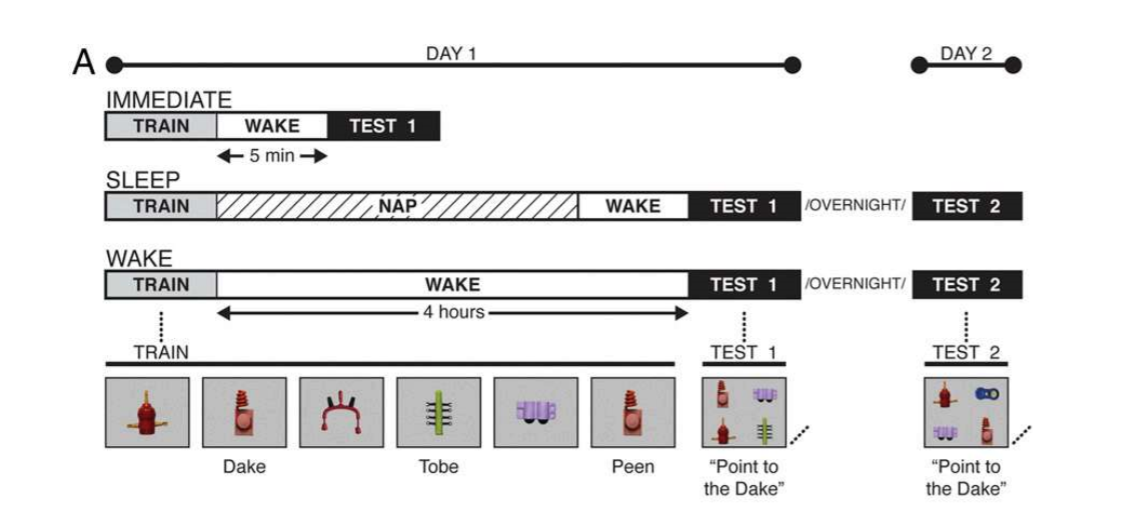
\includegraphics{C:/Users/mhorger/Documents/GitHub/Reproducible-Report_Horger/methods.PNG}
\caption{Methods}
\end{figure}

The goal of this study was to assess the retention of new words with
various intervals between training and test. Children received all
conditions 1-2 weeks apart. The conditions included: 1. after a 5 min
delay 2. after a nap (4 hour delay) 3. after 24 hours

\subsection{Data analysis}\label{data-analysis}

The authors assessed the number of trials needed to reach criterion
across conditions and groups.

The first analysis conducted was a repeated measures ANOVA for both wake
and nap conditions. The second was a 2x2 ANOVA with delay type as the
repeated factor and TD or DS as the between. These were conducted for
the 4 and 24 hour delay.

The second was a 2x2 ANOVA with delay type as the repeated factor and TD
or DS as the between. These were conducted for the 4 and 24 hour delay.

We used R (Version 3.5.2; R Core Team, 2018) and the R-packages
\emph{data.table} (Version 1.12.0; Dowle \& Srinivasan, 2019),
\emph{dplyr} (Version 0.8.0.1; Wickham, François, Henry, \& Müller,
2019), \emph{ggplot2} (Version 3.1.0; Wickham, 2016), \emph{papaja}
(Version 0.1.0.9842; Aust \& Barth, 2018), \emph{readxl} (Version 1.3.1;
Wickham \& Bryan, 2019), and \emph{xtable} (Version 1.8.3; Dahl, Scott,
Roosen, Magnusson, \& Swinton, 2018) for all our analyses.

\section{Results}\label{results}

\begin{tabular}{l|l|r|r}
\hline
Grouping & Timing & meanNTC & SEMNTC\\
\hline
DS & Immediate & 1.680000 & 0.2628054\\
\hline
DS & Sleep & 1.640000 & 0.1620699\\
\hline
DS & Wake & 2.080000 & 0.1993322\\
\hline
TD & Immediate & 2.041667 & 0.2789679\\
\hline
TD & Sleep & 1.708333 & 0.1408973\\
\hline
TD & Wake & 1.666667 & 0.2055980\\
\hline
\end{tabular}

\begin{figure}
\centering
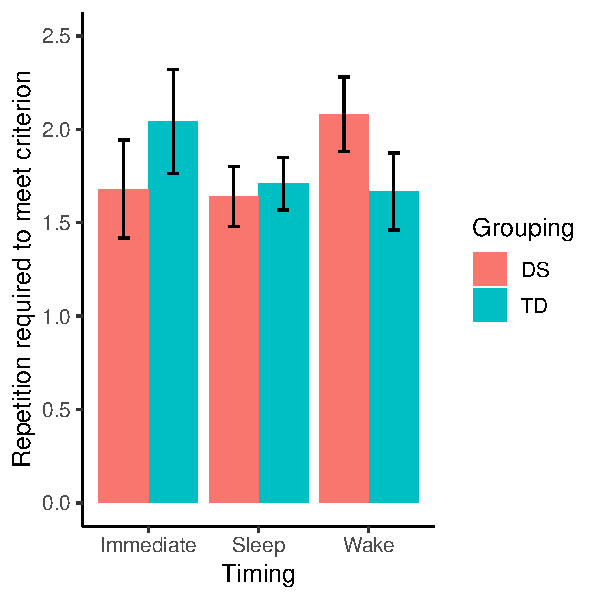
\includegraphics{Midterm_in_papaja_files/figure-latex/NumberToCriterion-1.pdf}
\caption{\label{fig:NumberToCriterion}Average number of trials to criterion
per group per condition.}
\end{figure}

{[}1{]} \enquote{factor}

Error: Subjects Df Sum Sq Mean Sq F value Pr(\textgreater{}F) Residuals
48 4.412 0.09192

Error: Subjects:Condition Df Sum Sq Mean Sq F value Pr(\textgreater{}F)
Condition 1 0.014 0.01372 0.049 0.825 Residuals 48 13.348 0.27808

Error: Within Df Sum Sq Mean Sq F value Pr(\textgreater{}F) Residuals 98
4.568 0.04661

\section{Discussion}\label{discussion}

\newpage

\section{References}\label{references}

\begingroup
\setlength{\parindent}{-0.5in} \setlength{\leftskip}{0.5in}

\hypertarget{refs}{}
\hypertarget{ref-R-papaja}{}
Aust, F., \& Barth, M. (2018). \emph{papaja: Create APA manuscripts with
R Markdown}. Retrieved from \url{https://github.com/crsh/papaja}

\hypertarget{ref-R-xtable}{}
Dahl, D. B., Scott, D., Roosen, C., Magnusson, A., \& Swinton, J.
(2018). \emph{Xtable: Export tables to latex or html}. Retrieved from
\url{https://CRAN.R-project.org/package=xtable}

\hypertarget{ref-R-data.table}{}
Dowle, M., \& Srinivasan, A. (2019). \emph{Data.table: Extension of
`data.frame`}. Retrieved from
\url{https://CRAN.R-project.org/package=data.table}

\hypertarget{ref-R-base}{}
R Core Team. (2018). \emph{R: A language and environment for statistical
computing}. Vienna, Austria: R Foundation for Statistical Computing.
Retrieved from \url{https://www.R-project.org/}

\hypertarget{ref-R-ggplot2}{}
Wickham, H. (2016). \emph{Ggplot2: Elegant graphics for data analysis}.
Springer-Verlag New York. Retrieved from \url{http://ggplot2.org}

\hypertarget{ref-R-readxl}{}
Wickham, H., \& Bryan, J. (2019). \emph{Readxl: Read excel files}.
Retrieved from \url{https://CRAN.R-project.org/package=readxl}

\hypertarget{ref-R-dplyr}{}
Wickham, H., François, R., Henry, L., \& Müller, K. (2019). \emph{Dplyr:
A grammar of data manipulation}. Retrieved from
\url{https://CRAN.R-project.org/package=dplyr}

\endgroup


\end{document}
